\chapter{Evolutionary dynamics on graphs}
\label{chp:nature} 

 

When investigating cyber insurance and insurable topologies, it is important not to only focus on standard risk networks, such as the internet. Our goal is to investigate all kinds of networks, or especially networks where players actions are influenced by their neighbourhood structure, i.e. the network connections will affect each individual players payoff. 
In this case there are several types of networks to consider, all social and economic interactions where an agents well being is dependent on externalities as well as her own actions, is a network worth considering network.

As mentioned earlier, the internet is a very good example, because on the internet we are "all" connected, the benefit we get from the internet is strongly dependent on this, and so is the risk we face when using the internet. 
Other examples could be the networks that are formed when a company are developing a software product, this development process is often done by several different firms, and thus creates a development network, where everyone is dependent on the result of the others. 
If one or more fail in some way, bankruptcy, failure to deliver at the expected time, higher cost etc. 
Then the whole network will be affected. 
Or in a cloud computing network, there are many different users and internet service providers, and the overall security is dependent on all of them. 
As we see all these networks are different from each other, some face direct connections, other consist of social and economical connections. But they all share some main characteristics, they are all experiencing network effects, externalities, information asymmetry, correlated risk and interdependent security. \cite{networkgames}

In our paper an insurable topology, is an network structure which makes it feasible for both the
 insurer(supply side)  to offer and the customer(demand side) to acquire insurance.
 For this to be possible there are many  difficulties to overcome,  one example are the correlated risks, from the insurers point of view, the problem is to be able to calculate the overall probability of casualty/infection, which can be very difficult without graph theory. 



 The paper \cite{lieberman2005evolutionary} is about evolutionary dynamics and how certain structures
can amplify or sustain evolution or drift\footnote{Drift is the opposite of selective evolution
, it is when the network/structure evolve and change at random}. To be able to find insurable topologies, an extensive study of different graphs and how they behave has to be conducted. Regarding security, knowledge of how viruses spread and how to use graph structures to prevent malicious hackers from entering your network is important. Evolutionary dynamics, and the research of how mutant genes spread though out a population is a very useful field when looking for an insurable topology. 
If one can determine some structures, where some nodes are advantageous/disadvantageous , then these structures will have certain properties, such as sustaining viruses from spreading, or amplify the incentive for obtaining cyber-insurance and
protection software. If one could identify these nodes and networks, then this information could  be used to determine if it is an insurable topology.

In the \cite{lieberman2005evolutionary} paper, they show that mutants inserted in to a
 circulation graph, will have a fixation probability equal to
\begin{equation}  p_{1}=\frac{(1-\frac{1}{r})}{(1-\frac{1}{r^{N}})} \label{eq:fixation} \end{equation}
Where $r$ represents the relative fitness of the mutant, if it is advantageous it will have a certain chance of fixation, and disadvantageous mutants will have a chance of extinction. 
A circulation graph is a graph that satisfy these two properties:
\begin{enumerate}
\item the sum of all edges leaving a vertex is equal for all vertexes
\item the sum of all edges entering a vertex i equal for all vertexes
\end{enumerate}
The fixation probability determines how probable it is that the whole network will eventually be
"infected" by the mutant. I.e. it determines the rate of evolution, which relies on both the size of the
network and the evolution speed. 
A probability equal to one means that every node in the network eventually will be affected by the mutant.
A circulation graph is not necessarily an insurable topology, but if we can find graphs with  fixation probability that exceeds equation \ref{eq:fixation} they could possibly be considered as insurable topologies, because if we can find these graphs, then it will be possible to suppress drift and amplify selection and visa versa. 
\begin{figure}[b]
\centering
\begin{tabular}{@{}c@{}}
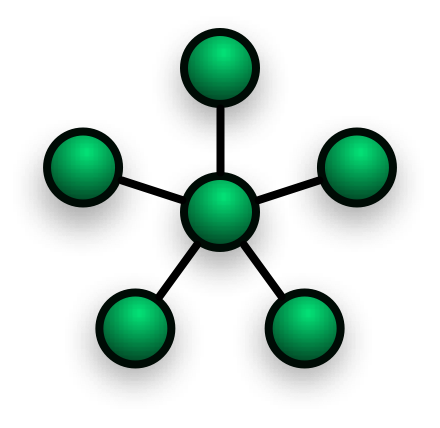
\includegraphics[width=0.5\textwidth]{NetworkTopology-Star.png}
\end{tabular}
\caption{
\label{fig:star} A star-topology 
\cite{lieberman2005evolutionary} . 
}
\end{figure}
The paper shows that there exists such graphs, one example is the star topology. (see figure \ref{fig:star})
In this topology the fixation probability is as shown in equation\ref{eq:fixation2}, or for more general see equation \ref{eq:fixationk} \begin{equation}p_{2}=\frac{(1-\frac{1}{r^{2}})}{(1-\frac{1}{r^{2N}})} \label{eq:fixation2} \end{equation}.
or more generall: \begin{equation}
p_{k}=\frac{(1-\frac{1}{r^{k}})}{(1-\frac{1}{r^{kN}})} \label{eq:fixationk}
\end{equation}
 When comparing the equations \ref{eq:fixation} and \ref{eq:fixation2}, we see that the selective difference is
 amplified from $r$ to $r^{2}$, i.e. a star act as an evolutionary amplifier, favouring advantageous
  mutants and inhibiting disadvantageous mutants.

There exists other graphs where the fixation probability is equal to \ref{eq:fixationk}, examples are super-stars, such as funnels and
metafunnels. These are just more complex star networks. This paper shows,  that the super-stars if N is large enough, the fixation probability for an advantageous mutant converges to 1, 
and for disadvantageous converges to 0. 
As we know from chapter \ref{chp:graphTheory}, there are many
topologies in our society that are so called scale-free. Scale-free networks have most of their connectivity clustered in a few verices, the star and the super-stars are all scale-free, and scale-free networks are potent selection amplifiers.

\subparagraph{Star-network as an insurable topology}
The paper \cite{networkgames} shows how network games evolve when the payoffs are determined not only by your own decisions, but also by your neighbours. This can be used to analyze the insurable-topology, star network, further. One of the games they analyzes is simple but highly relevant for our paper, a public goods game. A good example of a public goods is security product, because it suffers from strategic substitutes, i.e. if your neighbour acquire the security product, you have less incentive of also acquiring the security product, because when he acquire it, he gets more secure, but so do you, due to the positive externalities of the product.

Lets consider a simple game shown in this paper,
We have an action space: $X=\{0,1\}$, where 1 can be considered as acquiring information, take vaccine, buy security software etc. And 0 is not doing so.
Each node $i$ has a set of neighbours: $N_{i} $, and a payoff function $y_{i}=x_{i}+\bar{x}N_{i}$. 
The gross payoff to player $i$ is 1 if $y_{i}>=1$ and 0 otherwise. But each player also suffer from a cost of $0<c<1$ if they choose action 1.
%% [location]h-here, t top, b bottom.
\begin{figure}[h]
\centering
\begin{subfigure}{.4\textwidth}
  \centering
  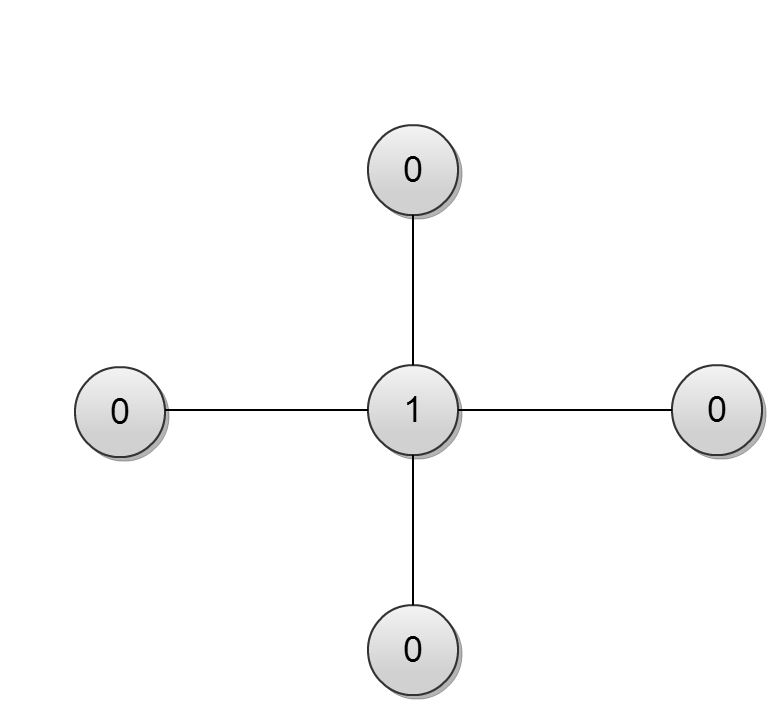
\includegraphics[width=0.8\linewidth]{optimalequilibrium.png}
  \caption{\label{fig:optequi} Socially Optimal equilibrium, center node choose action 1}
\end{subfigure}
\quad
\begin{subfigure}{.4\textwidth}
  \centering
  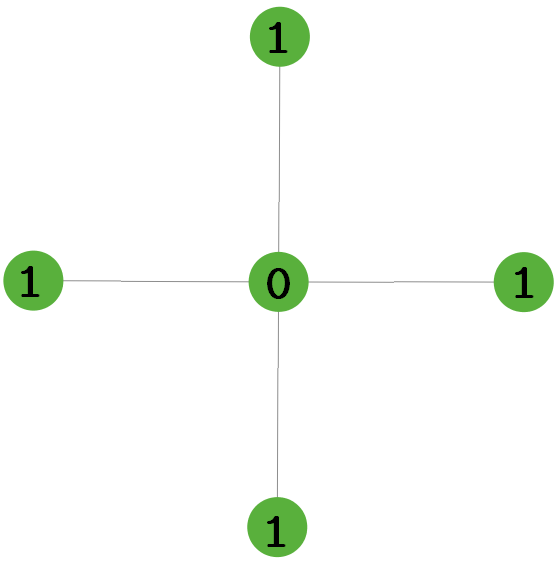
\includegraphics[width=0.8\linewidth]{notoptimalequilibrium.png}
  \caption{\label{fig:notoptequi} Non Socially Optimal equilibrium, leaf nodes choose action 1}
\end{subfigure}
\caption{\label{fig:starequi} Figure \ref{fig:optequi} shows the socially optimal equilibrium, and \ref{fig:notoptequi} shows the non optimal equilibrium.}

\end{figure}
When looking at \ref{fig:starequi}, we easily see that there is two equilibriums. One where the center node choose action 1 and the rest of the nodes choose action 0, and a second equilibrium where all the leaf nodes chooses 1 and the center choose 0.
The overall payoff in these two differ from each other, the latter is not socially optimal because it
 suffers from a cost equal to: $\#leaf nodes*c$ , the first equilibrium have a total cost of only $c$.
 It would have been very good if we where able to force the game to end up in the social optimal equilibrium.
\subparagraph{From a insurers point of view}
If a insurance company could identify these star-structures, and force them to end up in the social optimal equilibrium it would have been very beneficial for both the insurer and the customers.
First of all if the insurer could identify these structures, he could calculate the overall probability of fixation by a diseased mutant(virus, worm, trojan or other failures) as shown earlier. And if they could ensure that the center node is protected they could also calculate the probability of the diseased mutant being extinguished from the network.
One possibility of achieving this could be by offering very cheap insurance to the leaf nodes, and giving the center node an incentive to acquire security product, by informing the center node about the probability of failure unless he acquires security. And offer him a very good rebate if acquire the security product, and a very expensive insurance if not. In this way the insurer could force a rational center node to getting both insurance and security product, and thus securing the whole network.

This is a simple scenario, analyzing an exogenous network formation \footnote{Exogenous: The network formation is given. Endogenous: The structure originates from within the network, i.e. the oposite of exogenous}, 
but it shows how a insurer can, by using the results from \cite{lieberman2005evolutionary}, force the game to end up in the social optimal equilibrium, and also how the insurer can calculate the probabilities of failure. 
The contributes significantly to solving some of the problems with cyber-insurance. The problems with information asymmetry and interdependent risk problem has been reduced, since if the insurer knows the network structure, he can calculate the probabilities of failures and catastrophic events, the most important information he needs is how secure the center node is. If he also can ensure that the center node is secure, the interdependent risk problem is limited to only one node, the center node. All this result in a simple but insurable network topology.

   
\section{Notater og slikt}

\section{NOTES... random.. don't read}
 
The game:
The way this game works, is that we look at nodes that are mutated (A), and those who are not (B).  

When we apply the game to a directed graph, there are four different outcomes, a,b,c and d, which represents the interaction between the nodes, as is depicted in the figure below\ref{fig:game}. 

In the first figure (Positive symmetric) the fixation probability is related to r=b/c. If b is greater than c, the properties of mutant b will propagate in to all the other nodes, and the whole graph will eventually consists of only mutated nodes. The opposite will happen in the case where c is greater than b, leading to extinction of the mutation. The later scenario models the situation where proper protection against a mutant i.e. a security threat is installed. If the level of security, c is higher that the strength of the security threat it will be blocked from propagating further into the network. 


\begin{figure}[h]
\centering
\begin{tabular}{@{}c@{}}
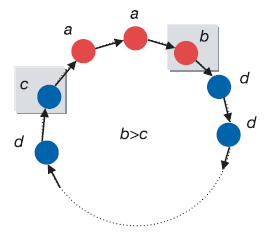
\includegraphics[width=0.5\textwidth]{natureGameSingle.png}
\end{tabular}
\caption{\label{fig:game} Mutant propagation game}
\end{figure}

More generalized, $W$ does not need to be stochastic, $w_{ij}>=0$. 
If the sum of all edges leaving a vertex is equal for all vertexes, then the graph will never suppress selection.
If the sum of all edges entering a vertex is equal for all vertexes, the graph never suppress drift.
If both then the graph is called a circulation.
     

Where the fixation probability determines the rate of evolution, which relies both on the size of the network and the evolution speed. A probability of 1 means that every node in the network eventually will be affected by the mutant.   
Isotherm graphs are a sub-graph of circulation. 

If $W$ is symmetric, or isotherm then the fixation probability is always \ref{eq:fixation}
isotherm means doubly stochastic, all rows and cols sum to 1. 
If a graph is one rooted, it has a fixation prob of $1/N$ regardless of $r$. If a graph has more then one root, its fixation probability is zero. 
Is it possible to find graphs with fixation probability that exceeds \ref{eq:fixation}? Is it possible to suppress drift and amplify selection?

